%!TEX root = thesis.tex

\chapter{Some Methodical Advice}
\label{chp:MethodicalAdvice}
In this chapter, I'll provide some methodical advice on writing and structuring the thesis document. Notably, this chapter provides you with extra sources on providing a meaningful and transparent structure of the thesis document.

~\\
\vfill
\minitoc
\clearpage


\section{Introduction}
\label{sec:03:Intro}
There are many tips and guidelines for writing good theses. Anyway, let me give you some very basic information first, before digging into the details.

First of all, there are excellent guidelines to conduct and report research. First and foremost, everyone should read Wohlin et al.~\cite{wohlin2012experimentation} to get a feeling for the very basics of conducting and reporting research. Wohlin's book is, however, a general guideline for Software Engineering. Other disciplines, e.g., Information systems favor other guidelines, e.g., Recker \cite{Recker2021}. For specific types of studies, however, there are further, more specialized books, articles, and guidelines that help structure the research in general and a thesis report in particular:
\begin{enumerate}
	\item General case study research, Runeson et al.~\cite{Runeson:2012aa,runeson09}
	\item Systematic literature reviews (SLR), Kitchenham et al.~\cite{Kitchenham:2015rt,Kitchenham:2004fk}
	\item Systematic mapping studies (SMS), Petersen et al.~\cite{PVK15}
	\item Survey research, Lin\r{a}ker et al.~\cite{Linaker:2015aa}
\end{enumerate}
Depending on the actual type of research you conduct, consult the respective guidelines first! Also, special attention should be given to \cite{Runeson:2012aa}, since this book provides a comprehensive and straightforward guideline for a general structuring of reports.

\begin{MySugg}
	It is also a good and straightforward idea to check for some ``older'' thesis reports. Your supervisors will for sure provide some\ldots
\end{MySugg}

\section{The Bachelor's Thesis Process}
\label{sec:03:ThesisProcess}
This section specifically addresses Bachelor's Theses\footnote{For detailed information regarding Master's Theses, please consult the Thesis Guideline and/or contact Prof. Decker.}, which require certain steps that are described in the following.

\paragraph*{Qualification} 
To start the Bachelor's Thesis, you have to fulfill certain requirements, notably, you have to have successfully passed the intermediate exam and you need to have obtained a minimum number of ECTS points. To show your ``formal qualification'', in the course of \emph{finding a topic}, you should export a transcript from the Campus Portal, which should be evaluated either by the desired supervisor or, if necessary, by the head of the examination board. At latest when it comes to the \emph{topic registration} (the official start), you need to present your qualifications.

\paragraph*{Supervisor Search} 
Potential supervisors for Bachelor's Theses are, basically, all examiners of the faculty, usually the professors. This also holds for theses that are conducted collaboratively with partners from industry. That is, you need to always find a responsible main supervisor, who is associated with the HHZ\footnote{In case you plan to conduct the thesis in Reutlingen, e.g., in the business faculty, please contact Prof. Breitenb\"ucher.}.

\paragraph*{Topic Search}
Closely linked with the supervisor search is the topic search---usually, these activities go hand in hand. Most of the HHZ professors offer multiple topics for Bachelor's Theses. You can also go for a specific topic for which you, usually, get the supervisor ``for free''. In case there is no appealing topic available, you can also directly approach a potential supervisor to discuss potential topics. Furthermore, there is also the opportunity to work on an industry-inspired topic. However, if you bring a topic from industry to the table, you also need to find a supervisor. \textbf{Important!} Please have in mind that the final topic assignment is the responsibility of the examiners. The university decides about the appropriateness of a topic \emph{not} an industry partner.

\paragraph*{On-Boarding Phase}
After the initial topic assignment, we usually grant an on-boarding period. The supervisor might also request creating an additional \emph{Exposee}. This phase mainly serves the students' critical self-evaluation, whether or not the ``right'' topic has been chosen. At the end of the on-boarding phase, you (1) either accept and register the provided topic, or (b) return the topic and select another one. \emph{The on-boarding phase is limited to 4 weeks}.

\paragraph*{Thesis Registration}
It is your responsibility to initiate the formal thesis registration. For this, there is a form available in the intranet that you execute together with your main supervisor. The second supervisor, which you need to find as well, confirms the registration with its signature. As soon as both supervisors have signed the form, you have to send the signed form via email to Prof. Breitenb\"ucher. 

\paragraph*{Conducting the Thesis Project}
The timeframe of the Thesis project is 4 months \textcolor{red}{\textbf{strict}}! The timeframe is defined with the starting and end dates as agreed with the supervisors and documented in the thesis registration. Within this timeframe, the actual work is conducted in the mode of work that the students and supervisors agreed upon. The Thesis project is time-boxed---any deviation and/or extension requires a significant reason and an application.

\paragraph*{Colloquium}
In the course of conducting the Thesis project, you have to participate in the Colloquium. In every semester, there are usually two time slots, which are announced in advance. You have to attend at least one Colloquium (a registration is required), and you have to participate in the whole Colloquium session, i.e., full participation is mandatory.

\begin{MySugg}
	You should consider attending two or more Colloquium sessions as these might help you understand what's important and what to pay attention to\ldots
\end{MySugg}

\section{General Structure of a Thesis}
\label{sec:03:ThesisStructure}
There are many approaches to structure a thesis. However, the very basic report outline should look as follows:
\begin{enumerate}
	\item Introduction
	\item Background and Related Work
	\item Research Design
	\item (Your specific content as needed)
	\item Conclusion
\end{enumerate}
The fine-grained structure, however, depends on your actual type of work (see the guidelines above). Nevertheless, there are few further suggestions.

\begin{MySugg}
	There is one \emph{really important remark}: Meanwhile, there are (quasi-)standards regarding the way of conducting and reporting scientific work. That is, certain study types dictate specific document structures. For instance, if you conduct a systematic literature review, there are standards that must be followed. Likewise for experiments and action research. Eventually, your supervisor will help you defining the thesis document's outline. However, be aware of the standard procedures available as ignoring those standards might lead to downgrading your work.
\end{MySugg}

\begin{MySugg}
	Another remark: to get some inspiration of what to write where, read some selected (scientific) articles related to you thesis topic. Such articles usually provide good advice which information is required to be presented where in the document. In case there are variations---there will be variations---consult your supervisor to find the best-fitting solution.
\end{MySugg}

\subsection{Extended Structuring}
\label{sec:03:ThesisStructure:ExtendedStructuring}
There are for instance scientific journals that ask their authors to provide a so-called \emph{structured abstract}. Well, I'm not a fan of structured abstracts---abstracts shall be some sort of appetizer and thus should be ``nice'' and not over-engineered, even though there are good reasons for structured abstracts. So, my recommendation is to not use structured abstracts\ldots

And here is the BUT: But the introduction chapter of your thesis should be structured. And for structuring the introduction, the following approach has become a best practice. Provide a structure for the introduction as follows:
\begin{itemize}
	\item At first, provide a motivation text that sets the scene for your work.
	\item Provide a subsection or a paragraph (use the respective \LaTeX-commands) for the \emph{Problem Statement}, and describe the problem properly.
	\item Provide a subsection or a paragraph for the \emph{Objective} of your work. Please be aware of the fact that the the overall objective is \emph{not} your research question! It's the objective of the overall piece of work that you provide. The research questions have to be provided in the research design section.
	\item Provide a subsection or a paragraph for the \emph{Context} of your work.
	\item Provide a subsection or a paragraph for the \emph{Contribution} of your work.
	\item Provide a subsection or a paragraph for the \emph{Outline} to guide the reader through your work.
\end{itemize}
Please be aware that the introduction lays the foundation for the work. So, you should clearly state \emph{why} you do this work and \emph{what} is the outcome of the work.

\begin{MySugg}
	In general, as a rule of the thumb, the introduction should not exceed 3-5 pages. Keep everything short and clear!
\end{MySugg}

\subsection{Writing and Style}
\label{sec:03:ThesisStructure:WritingStyle}
Important for writing a thesis is also that you are able to convey a message. Hence, make your points. Do it clearly and do it concisely! In the following, there are some standard suggestions grounded in the many student projects I have supervised so far.

\begin{labeling}{Long Sentences}
	\item[No Slang] A thesis report is a formal document. Therefore, it must not be ``boring as hell'', but, ensure you keep a certain level of professionalism in the writing.
	\item[Long Sentences] There is a difference between a \emph{sentence} and a \emph{paragraph}. A paragraph is  a collection of sentences. That is, avoid writing long and overly complex sentences that are paragraphs on their own. Use short sentences. Use a clear language.
	\item[False Friends] If you are not a native English speaker, be aware of so-called \emph{false friends}. Many metaphors and phrases common in your Mother's tongue are different---if they are present after all---in English. Use a context-based dictionary, e.g., \url{https://www.linguee.de}, to find the correct translation and the correct use of a translation variant in the respective context.
	\item[Stacking] Don't stack headlines, e.g., 1. X, new line, 1.1 X1, new line, 1.1.1 X11, and so forth. This is very bad style! Use glue text to separate the headlines. A good idea for such glue text is to provide a short description of the content to come, i.e., to inform the reader what comes next.
	\item[We or I] Basically, it doesn't matter. It depends on the characteristics of the work, and on how much you collaborated in the course of conducting your research. The ``safe'' way is using ``we''.
\end{labeling}
Also: even if you are a native speaker, consult somebody for proof reading and checking your report (also for German writing!). At best, you ask somebody who is not familiar with the topic. This way, you'll also get feedback if the clarity of the text is good enough for understanding the content even for persons outside your area of expertise.

\section{Technical Environment}
\label{sec:03:TechnicalEnvironment}
One important aspect: Don't use ``exotic'' technical environments. Keep your \LaTeX-environment slim (cf.\ Section~\ref{sec:1:LaTeX}). Don't use exotic tools. This doesn't make you ``cool''---it only ensures that your supervisors cannot share data or collaborate and help you. Use standard tools, whether you like them or not. Also, create and maintain your literature database with a tool. Don't write the items manually---this will only end up in you spending nights searching for missed commands and parentheses\ldots

\section{Frequently Asked Useless Questions}
\label{sec:03:FUQ}
Also, it happens more often than you would expect it, there are questions that are just useless. Nevertheless, I try to answer these questions to some extent:

\emph{Question: How many reference items do I need?} Well, as many as you need. It's quite simple: for some research projects, there is a lot of background material. When you compile your related work and shape your line of argumentation, you have to ensure that all statements, agreements and even claims are backed up by literature. That is, the number of items in your literature library is defined by the topic and the way you present your topic.

\begin{MySugg}
	As long as we're up: Wikipedia is no acceptable source for scientific statements. If you use Wikipedia, use it as a starter and---IMPORTANT---scroll down to the very end of the page where the actual references are listed. So, you may start with Wikipedia, but you are expected to go beyond Wikipedia and to inspect the actual scientific references. Also, as long as you don't do a \emph{Gray Literature Review} (GLR), websites, blogs, and so forth do also not count as acceptable references. You might refer to such sources for underlining certain statements in the text. In such cases, refer to those sources as footnotes.
\end{MySugg}

\emph{Questions: How many pages do I need to write?} Well, as many as you need, again. In fact, there is no absolute measure what the minimum number of pages (which is, to be honest, a fairly crappy metric anyway) you need to pass. Every topic has its individual requirements. It might happen that you work on a topic, write down 60 pages and your are done. There might be another topic that requires you to write 90 pages. Anyway, using \emph{\underline{this template}}, I can provide few experience-based numbers. But, these numbers are only average numbers and don't indicate to good or bad marks.
\begin{itemize}
	\item Bachelor's Thesis: between 50 and 70 pages (PDF-pages, in total)
	\item Master's Thesis: between 70 and 100 pages (PDF-pages, in total)
\end{itemize}
If you write more than 100 pages, you have to critically assess your document if everything you write is really necessary and contributes to the overall story. A ``chatty'' text usually only lowers the quality. So, make your point, write what is necessary, and not more.

\emph{Question: Do I really have to re-draw the figures?} Yes! This is your work and, therefore, you have to provide the basic content. Of course, there are always complex figures that are provided in other papers or in the web. In this case, when you plan using such material, ensure that all obligations regarding the copyright and intellectual property have been respected.

\begin{MySugg}
	Note that ``just using and placing stuff'' from other sources is plagiarism, and note that in the scientific community, plagiarism is a capital delict. Every institution and every supervisor implement specific procedures to handle plagiarism. So, don't ride this train---you risk your work!
\end{MySugg}

\emph{Question: What do I need to do to get an excellent grade?} Well, just do your work. Ensure you work according to good scientific standards and always have in mind that, especially, a Master's Thesis is an individual performance. That is, you have to organize and run the project independently. Eventually, the final grade is composed of a number of weighted components, which are shown in Figure~\ref{fig:gradingschema}. This grading schema might serve as a reference.

\begin{figure}[ht]
	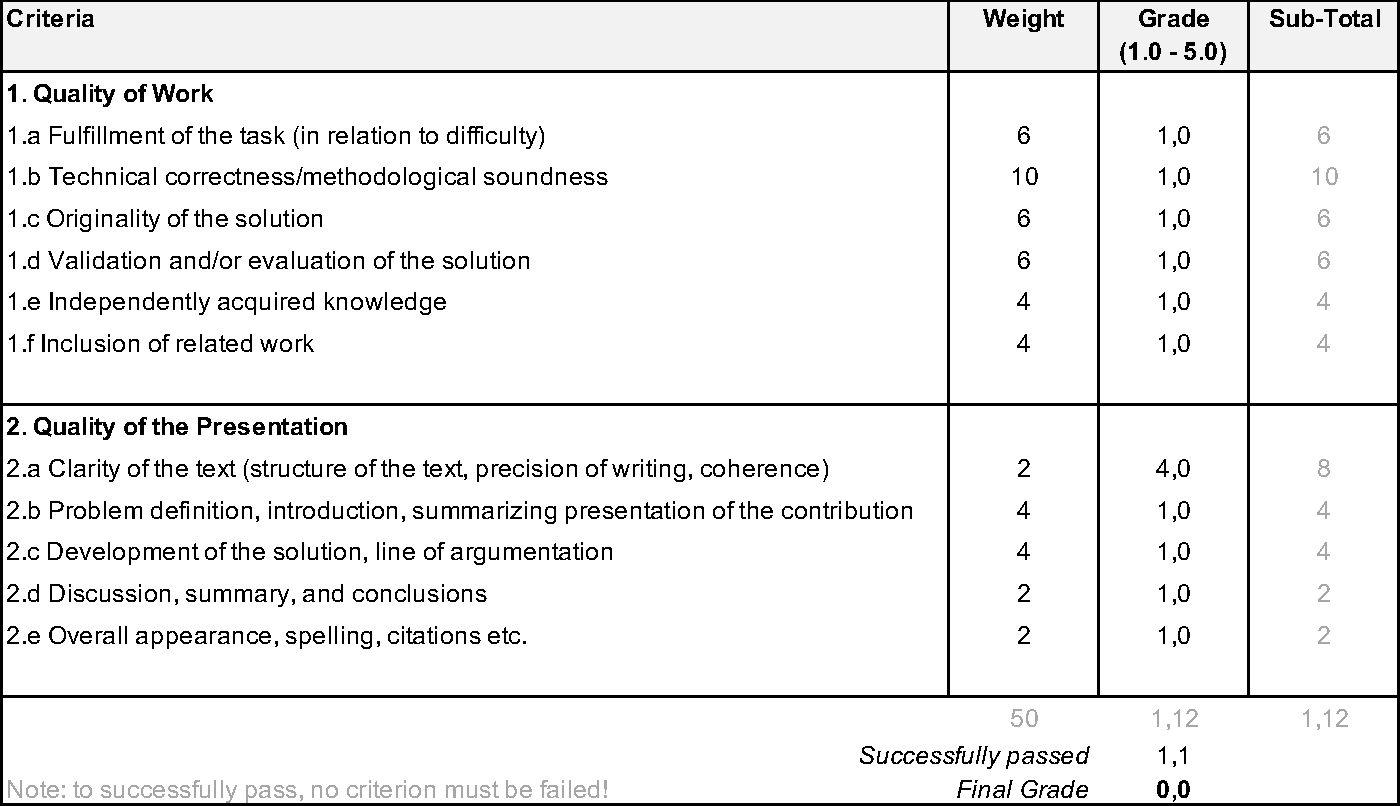
\includegraphics[width=1.00\textwidth]{figs/grading.pdf}
	\caption{Latest grading schema as a reference (2023)}
	\label{fig:gradingschema}
\end{figure}

\begin{MySugg}
	Again, to make this point clear: a Bachelor Thesis is a first scientific work, which is supported by supervisors to some extend. Yet, a Master's Thesis is a project in which you demonstrate that you can solve a given problem yourself. Of course, you will always receive support via discussions, reviews, feedback, and the like. However, if you start trying to get the supervisor's approval for every single sentence or if you come to a meeting unprepared asking a supervisor stuff that a simple Google search would have revealed in less than 10 seconds, you might see your work downgraded as your independent and/or self-directed/-organized work does not suffice.
\end{MySugg}

\emph{Question: Do I really have to use \LaTeX?} Standard: Yes! Anyways, discuss this with your supervisor since some might accept using something else, but then, everything is up to you\ldots

\emph{Question: The template is in English, so is English mandatory or can I also write the thesis in German?} The template is in English for only one reason: Pure and personal laziness. If you and your supervisor decide that the thesis shall be written in German, then the thesis is going to be written in German. In this case, you only need to change the language in the file \kw{thesis.tex}. In line 3 of the main file, you need to change the attribute \kw{english} in the \kw{documentclass} command.


%%% Local Variables: 
%%% mode: latex
%%% TeX-master: "thesis"
%%% End: 